% Chapter 1

\chapter{Introduction} % Main chapter title

\label{1.} % For referencing the chapter elsewhere, use \ref{Chapter1} 

%----------------------------------------------------------------------------------------

% Define some commands to keep the formatting separated from the content 
\newcommand{\keyword}[1]{\textbf{#1}}
\newcommand{\tabhead}[1]{\textbf{#1}}
\newcommand{\code}[1]{\texttt{#1}}
\newcommand{\file}[1]{\texttt{\bfseries#1}}
\newcommand{\option}[1]{\texttt{\itshape#1}}


%----------------------------------------------------------------------------------------


With the rise of the Internet of Things (IoT) and ever more sensors, gadgets and smart devices like smartwatches for fall detection or blood pressure monitoring, or fridges for temperature protective control in use, the amount of available data steadily increases \parencite{Alansari2018}. Simultaneously, the possibilities to use the data to draw conclusions increases. This data is generally used to draw conclusions such as failure of a system or a medical issue, such as a heart attack. These events typically occur very rarely \parencite{Hauskrecht2007}. However, when the number of instances of each class is approximately equal, most machine learning algorithms function best. Problems occur when the number of instances of one class greatly exceeds the number of instances of the other. This issue is very popular in practice, and it can be observed in a variety of fields such as fraud detection, medical diagnosis, oil spillage detection, facial recognition, and so on \parencite{Thabtah2020}. The task of identifying the rare item, event or observation is often referred to as anomaly detection. Typically, the anomalous item translates to problems such as bank fraud or medical problems. Often, the anomaly does not adhere to the common statistical definition of an outlier. Therefore, many outlier detection methods (in particular unsupervised methods) fail on such data \parencite{Hodge2004}

A special disciplin in anomaly detection is to find the anomaly in a time series. The anomaly detection problem for time series is usually formulated as finding outlier data points relative to some standard or usual signal. Time series anomaly detection plays a critical role in automated monitoring systems. It is an increasingly important topic today, because of its wider application in the context of the Internet of Things (IoT), especially in industrial environments. The most popular techniques to find the anomalies are:

\begin{itemize}
	\item Statistical Methods
	\item Support Vector Machines
	\item Clustering 
	\item Density-based Techniques
	\item Neural Networks 
\end{itemize}

Currently Neural Networks are regarded the cutting-edge research. Although first approaches to use artificial neural networks exist since 1969. They are popular in research for only about 15 to 20 years, which is why scientist generally expect further improvements on this kind of technology. This promising outlook is why this research paper also purely focusses on Neural Networks for anomaly detection. Especially Recurrent Neural Networks and Convolutional Neural Networks are investigated and compared. 

\section{Definitions}
Following, the most important terms in the context of anomaly detection using neural networks are elaborated and defined. 

\subsection{Univariate, Bivariate and Multivariate Data}
Time series data investigation poses a special disciplin. Generally anomalies in time series are harder to detect for traditional statistical models, since the possibility of long term dependencies exist. Time series data comes in different forms. It is distinguished between univariate, bivariate and multivariate data. Univariate involves the analysis of a single variable while bivariate and multivariate analysis examines two or more variables.

\subsubsection{Univariate Data}
There is only one variable in this type of data. Because the information only deals with one variable that changes, univariate data analysis is the simplest type of analysis. It is not concerned with causes or relationships, and the primary goal of the analysis is to describe the data and identify patterns.

\subsubsection{Bivariate Data}
This type of data involves two different variables. This type of data analysis is concerned with causes and relationships, and the goal is to determine the relationship between the two variables.

\subsubsection{Multivariate Data}
Multivariate data is defined as data that contains three or more variables. It's similar to bivariate, but there are more dependent variables. The methods for analyzing this data are determined by the objectives to be met. Regression analysis, path analysis, factor analysis, and multivariate analysis of variance are some of the techniques.

\textcolor{red}{
An example of a multivariate time-series is the collected data from several sensors installed in a car.
One main difference between time-series and other datasets is that the observations do not only depend on components
d, but also on the time feature n. Thus, time-series analysis and the used statistical methods are mostly different from
the methods used for random variables that assume independence and constant variance of the random variables.
To data analysts, time-series are important in a variety of fields like economy, healthcare and medical research, trading,
engineering and geophysics. These data are used for forecasting and anomaly detection.}


\subsection{Neural Networks}

An Artificial Neural Network (ANN) with several layers between the input and output layers, is known as a Deep Neural Network (DNN). Neural networks come in a variety of shapes and sizes, but they all have the same basic components: neurons, weights and functions. These components work in a similar way as human brains and can be trained just like any other machine learning algorithm.

\subsubsection{Neuron}
Artificial neurons represent the smallest building blocks of neural networks. A neuron usually receives separately weighted inputs which it sums. The sum is then passed through the activation function to calculate the output of the neuron. When training a neural network, the input weights are adjusted by the optimizer function to improve accuracy of the given task e.g. classification.

\subsubsection{Layer}
In neural networks three different kind of layers are distinguished. There are input, output and hidden layers. A layer can be described as a collection of neurons. All layers between the input and output layer are called hidden layers. In the input layer data is fed into the neural network. The output of the hidden layer is calculated by taking the weighted sums of input and passing it through the activation function. Typically, a more complex problem requires more hidden layers to accurately calculate the output. In the output layer the final result e.g. a classification is produced. Figure \ref{fig:layers} how a simple Neural Network with just one hidden layer could look like.


\begin{figure}[h]
	\centering
	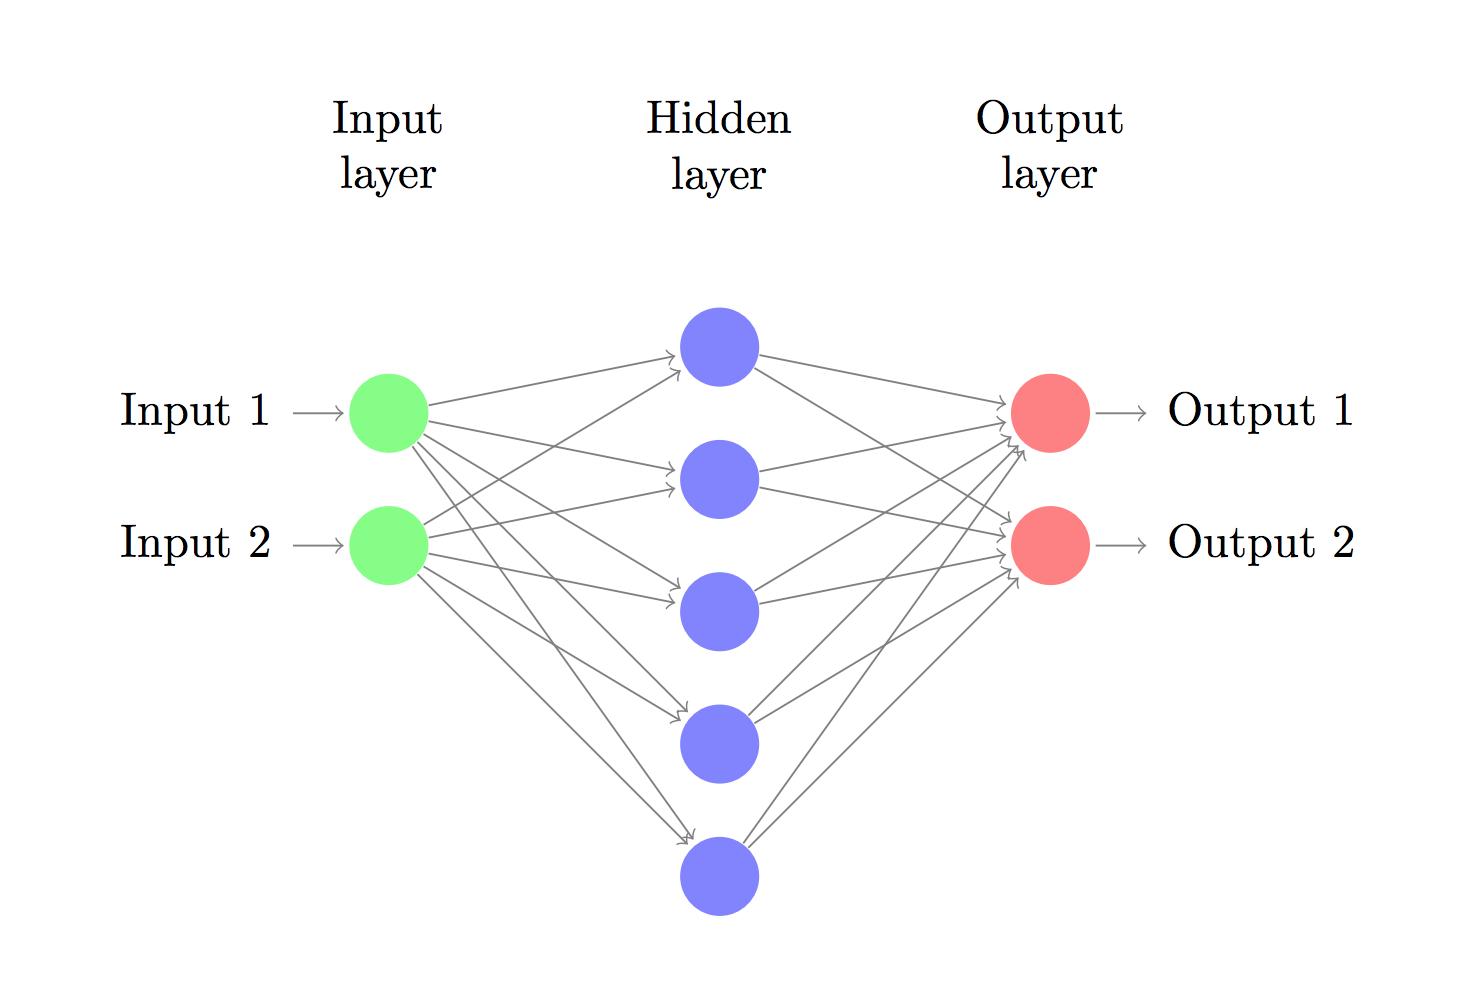
\includegraphics[scale=0.3]{Figures/layers}
	\decoRule
	\caption[Layers]{Input, Hidden and Output Layers \parencite{DennyBritz2015}}
	\label{fig:layers}
	%https://blog.csdn.net/mydear_11000/article/details/51087980
\end{figure}



\subsubsection{Optimizer Function}


\section{Background}

Following, it is explained how different kinds of neural networks work and what they are used for.

\subsection{Neural Networks for Anomaly Detection} \label{NN}

Out of the three most popular neural network architectures, convolutional neural networks (CNN), recurrent neural networks (RNN) and deep neural networks (DNN), only RNN are typically used for anomaly detection in time series. RNNs have built-in memory and are therefore able to anticipate the next value in a time series based on current and past data. Classic or vanilla RNNs can theoretically keep track of arbitrary long-term dependencies in input sequences. There, however, is a computational issue: when using back-propagation to train a vanilla RNN, the back-propagated gradients can "vanish" or "explode" due to the computations involved in the process, which use finite-precision numbers. Because LSTM units allow gradients to flow unchanged, RNNs using LSTM unit or Gated Recurrent units (GRU) partially solve the vanishing gradient problem and therefore drastically improve accuracy.

Specially to mention in this context are LSTM (Long-Short Term Memory) and GRU (Gated Recurrent Units). Both achieved outstanding performance when used for tasks such as unsegmented, connected handwriting recognition, speech recognition and anomaly detection in network traffic or IDSs (intrusion detection systems) \parencite{JunyoungChung2014}

\subsubsection{LSTM} \label{LSTM}
LSTM was first proposed in 1997 by Schmidhuber and Hochreiter \parencite{Hochreiter1997}. The initial version to the LSTM unit consisted of a cells, input and output gates. In 1999, the LSTM architecture was improved by introducing a forget gate and therefore allowing the LSTM to reset its own state \parencite{Gers2000}. LSTM is used in a supervised training approach, that means it tries to predict a predefined state taking the past and the current state. If the predicted state differs from the expected state, the weights of the different gates are adjusted using an optimizer algorithm such as gradient descent. Figure \ref{fig:LSTM} shows how the gates and the cell are arranged. The cell represents the memory of the LSTM. In simple words, the LSTM works as follows to predict a new value: 

\begin{enumerate}
	\item Forget Gate: Obsolete information is removed from the cell state.
	\item Input Gate: New information is added to the cell state
	\item Output Gate: The new information and the cell state are added to make the new prediction.
	\item The new cell state is propagated to the next LSTM unit  
\end{enumerate}
     
\begin{figure}[h]
	\centering
	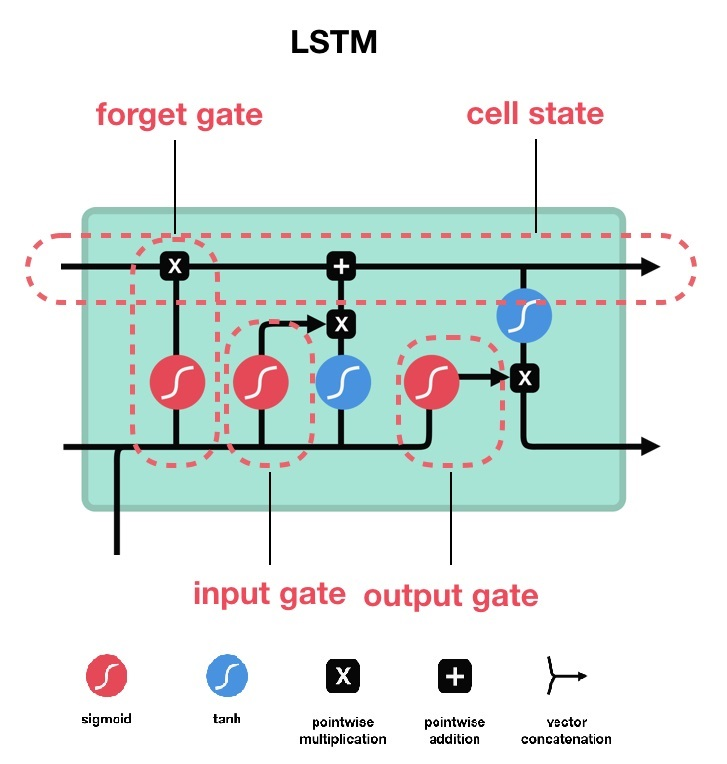
\includegraphics[scale=0.5]{Figures/LSTM}
	\decoRule
	\caption[LSTM]{Gates and Cell of LSTM  \parencite{MichaelPhi2018}}
	\label{fig:LSTM}
\end{figure}

% from https://towardsdatascience.com/illustrated-guide-to-lstms-and-gru-s-a-step-by-step-explanation-44e9eb85bf21

%\subsubsection{GRU}
% maybe not necessary

\subsubsection{CNN}
In contrast to RNNs Convolutional Neural Networks are generally used for image classification. CNNs work as feature extractors and are able to recognize patterns. CNNs use layers that are not fully connected, to reduce complexity (compare to \ref{NN}). In a CNN, a set number of neurons forms a filter. These filters or kernels are the actual feature extractors. A filter may represent a line or pattern (see Figure \ref{fig:filter}).\parencite{Aggarwal2013}

\begin{figure}[h]
	\centering
	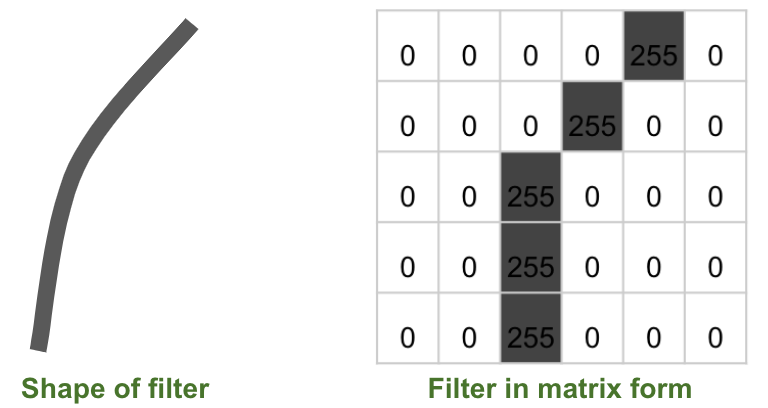
\includegraphics[scale=0.7]{Figures/filter}
	\decoRule
	\caption[Kernel]{Example of a Filter used in CNN}
	\label{fig:filter}
\end{figure}

To detect whether, a feature is occurrent in a picture, the filter is gradually moved over the picture in so called strides. In every step (stride) the dot-product between the filter and the part of the picture is calculated. The results of the operations are stored in activation maps.  The greater the dot-product the more alike are the filter and the section of the image. Training the network hereby refers to determining the shapes of these filters.
Other typical features of a CNN are the pooling layers. The pooling layers reduce the amount of computation necessary. The most commonly used pooling technique is max-pooling and works as shown in Figure \ref{fig:pooling}.

\begin{figure}[h]
	\centering
	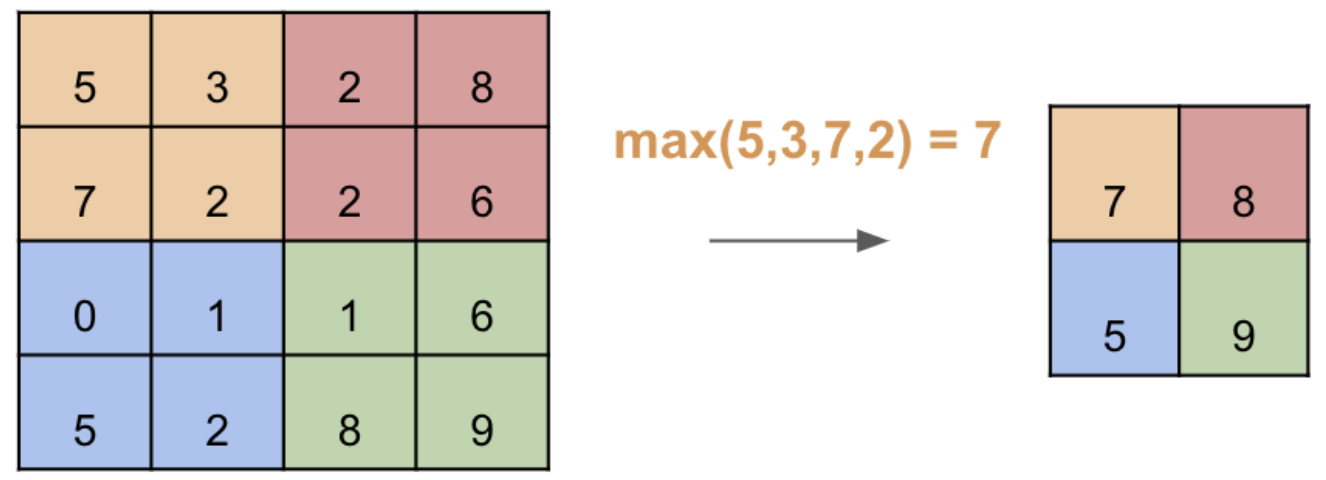
\includegraphics[scale=0.2]{Figures/pooling}
	\decoRule
	\caption[Pooling]{Example of max-pooling}
	\label{fig:pooling}
\end{figure}

The idea of max-pooling is to only keep the maximum value of an activation map. In the orange region 7 represents the maximum value, so it is kept while the other values are discarded \parencite{RichStureborg2019}.

In 2019, Wen and Keys proposed to use CNN also for anomaly detection in time series since it shares many common aspects with image segmentation. A univariate time series is therefore viewed as a one-dimensional image.\\ 


% https://towardsdatascience.com/conv-nets-for-dummies-a-bottom-up-approach-c1b754fb14d6


\subsection{Transfer Learning}
%https://builtin.com/data-science/transfer-learning
%Section about transfer learning\\
The reuse of a previously trained model on a new problem is known as transfer learning. It is currently very popular in deep learning because it can train deep neural networks with a relatively small amount of data. This is particularly useful in the field of data science, as most real-world problems do not provide millions of labeled data points to train complex models.
In transfer learning, the knowledge of an already trained machine learning model is applied to a different but related problem. For example, if a classifier was trained to predict if an image contains a backpack, the model's experience could be applied to recognize other objects such as sunglasses \parencite{NiklasDonges2020}.

\section{Problem Statement}

Defining a ground truth is one of the most difficult aspects of time series anomaly detection. Determining when anomalous behavior begins and ends in time series is a difficult task, as even human experts are likely to disagree in their assessments. Furthermore, there is the question of what constitutes a useful detection when detecting anomalies in time series.
In the past, RNN have successfully been used for anomaly detection (e.g. [Malhotra et al., 2015; Kim et al., 2016; Wang et al., 2017; Yin et al., 2017]. Therefore, designs for various use cases are well researched. RNN are well suited for the task, however, take a long time to train due to the complexity of how a single unit is designed (see \ref{LSTM}). In comparison CNN are not as complex and therefore, generally take less time to train. However, CNNs are generally used for image recognition and were only very recently used for anomaly detection in time series. It is therefore mostly unknown what designs are applicable for successful anomaly detection in time series data. %is this true?
While RNN are able to deal with multivariate data by design, a classical CNN requires design changes to be able to deal with multivariate data. Wen and Keys \parencite*{Wen2019} proposed to use a special kind of U-net, an improved version of a Fully Convolutional Neural Network \parencite{Ronneberger2015}.
Further, a CNN is not capable to analyze streaming data so it relies on segmentation of the data. These data segments are called snapshots. In order to not miss any data points, the frequency of taking these snapshots should be at least as high as the length of snapshot so that every time point is evaluated by the model at least once. However, for better performance it might prove beneficial to use a higher frequency which means every point is evaluated various times by the model \parencite{Wen2019}. The proposed design change and the fact that every point is evaluated multiple times, increases complexity and evaluation time and therefore counteract the architectural advantage of CNN compared to a RNN. 
When designing a neural network many parameters have to be chosen, this applies to both mentioned types of Neural Networks. For example, when designing a CNN, the number of layers, the activation function(s) of a single neuron and the optimizer function have to be chosen. Additionally, when using CNN for time series data the length and frequency of the snapshots have to be determined. Similarly, when designing a RNN also the number of layers and the optimizer function have to be determined. Because the basic building blocks of both networks types are very different it is difficult to fairly compare the complexity of two architecture approaches. Another important parameter which applies to both network types is the number of epochs for which the networks are trained. Through the epochs the training time is determined. In order to compare the two types of neural networks, two networks of similar complexity have to be designed. With equal training time the performance of both can be compared and evaluated. A RNN is therefore only set up as benchmark while the main goal of this research project is to clarify whether CNNs are really useful and propose an advantage over RNNs when applied on time series data for anomaly detection.

%transfer learning is missing

\section{Thesis Statement}

Convolutional Neural Networks are superior to Recurrent Neural Networks when looking for anomalies in time series data regarding training time and complexity.

\subsection{Subquestions}

\begin{itemize}
	\item How does a CNN for univariate and multivariate data need to be designed for successful anomaly detection in time series data?
	\item What advantages and disadvantages arise when using a CNN compared to a RNN for anomaly detection in univariate and multivariate time series?
	\item What parameter settings are crucial for a fair performance comparison between RNN and CNN? 
	\item Optional: How does transfer learning affect the performance of CNN compared to RNN in anomaly detection in time series?
\end{itemize}

 
\subsection{Research Objectives}

Following the research objectives of this paper are defined.

%always start with a verb ... to test, to determine

\begin{enumerate}
	\item Determine what design changes a CNN requires to detect anomalies in time series data.
	\item Determine how the CNN should be designed for the comparison with a RNN
	\item State the advantages and disadvantages of the chosen CNN architecture.
	\item Define parameters which allow a fair comparison of CNN and RNN
\end{enumerate}

\subsection{Limitations}

Recently there have been approaches that combine CNN and RNN into a hybrid network for tasks such as handwriting recognition or video-based emotion recognition \parencite{Dutta2018} \parencite{Fan2016}. However, this paper only compares pure CNN and RNN, and does investigate a hybrid approach.

% AUC and ROC not explained
% Test and training not explained 

\subsection{Significance}

Until now, time series data was almost only approached with RNNs. This paper should answer the question whether CNNs propose a valid alternative and even propose some advantages over RNNs. The paper will answer the fundamental question whether research should channel efforts to further investigate CNNs for anomaly detection in time series data or whether no benefits can be discovered and research is better to focus on other areas. 

\subsection{Chapter Overview}


%----------------------------------------------------------------------------------------
